\documentclass[conference]{IEEEtran}

\usepackage{graphicx}
\usepackage{subfig}
\usepackage{url}
\usepackage{algorithm}
\usepackage{algorithmic}
\usepackage{listings}
\usepackage{amsmath}
\usepackage{amsthm}
\usepackage{verbatim}
\graphicspath{{../figures/shm/}{../simulation/shm/}}
\newcommand{\HRule}{\rule{\linewidth}{0.5mm}}
\newcommand{\figurecurrentwidth}{\includegraphics[width=.49\textwidth]}
\newcommand{\figurehalfwidth}{\includegraphics[width=.24\textwidth]}
\lstset{float, numbers=left, frame=lines, belowcaptionskip=3mm, xleftmargin=7mm, framexleftmargin=7mm, escapeinside={(*}{*)}, tabsize=3, breaklines=true}
\newtheorem{theorem}{Theorem}
\renewcommand{\algorithmicrequire}{\textbf{Input:}}
\renewcommand{\algorithmicensure}{\textbf{Output:}} 
\begin{document}

\title{PSWare: A Flexible Middleware Framework for Composite Event in Wireless Sensor Network}
\author{
{Scribus Primus}\\
\affaddr{Primus Address}\\
\email{primus@somewhere.com} \and
{Scribus Secundus}\\
\affaddr{Secundus Address}\\
\email{secondus@elsewhere.com}
}
\conferenceinfo{SenSys'11,} {November 1--4, 2011, Seattle, WA, USA.}
\CopyrightYear{2011}
\crdata{XXX-X-XXXXX-XXX-X}
\maketitle
\begin{abstract}
Event detection is an important topic in many WSN applications. Although there are several works on providing event-based services in WSN, most of them can only deal with primitive event types but cannot handle composite events very well. In general, a type-based event system may have primitive or composite event types. All event types are defined by specifying their attributes and filters. Then, individual events are detected and delivered according to such type information. Composite event types may be defined by combining multiple event types with operators. Due to the resource constraints in WSN, composite events are much more difficult to manage than primitive events. In this work, we introduce PSWare, a type-based publish / subscribe middleware for WSN that supports composite events. We describe our design for PSWare. PSWare has a flexible architecture where different composite event detection algorithms may be easily integrated.

On top of PSWare, we present TED (Type-based Event Detection), a novel distributed composite event detection algorithm. The essential idea of TED is event fusion, where some sensor nodes are selected as fusion points and component events are fused for the detection of a high level event. Event fusion with minimum energy cost is an NP-complete problem. Therefore, TED uses a number of heuristics with bounded performance.  

To further increase the performance of event detection, we design a clustering algorithm for PSWare for structural health monitoring applications (SHM). We formulate the problem and found it to be NP-complete so we propose heuristic centralized and distributed algorithms. In addition to SHM, We use PSWare to develop other real world WSN applications including intelligent transportation system (ITS) and in-door monitoring.

We evaluate our system from different aspects. We first evaluate TED, the most essential algorithm in our system. We analyze its performance and then carry out extensive simulations. Both analytical and simulation results show TED can save energy in event-based applications where primitive events occur in a higher frequency than composite events. Then we combine TED with PSWare and carried out some real world experiments. The results show that PSWare can offer reasonably simple API for the application developers to use while TED and our clustering algorithm can improve the underlying event detection performance. Compared with opportunistic approaches to event detection in these real applications, PSWare can reduce 40 - 50 \% of the energy cost.
\end{abstract}
\chapter{Introduction}
\section{Overview}
\label{sec:introduction}
Development in wireless communication and electronics has made it possible to create low-cost, low-power wireless sensor nodes. Each sensor node usually contains a wireless transceiver, a micro processing unit and a number of sensors. The sensor nodes can collect data and do some simple processing locally, and can communicate with each other to form an ad hoc wireless sensor network (WSN) \cite{aky:survey}. A WSN is usually self-organized and self-maintained without any human intervention. Wireless sensor networks have been used in various application areas such as smart building \cite{lynch:shm}, wild environment monitoring \cite{wsnhabitat}, intelligent transportation systems \cite{klein:its}, battle surveillance \cite{wsntracking} and healthcare \cite{lo:ban}. 

While WSN has a wide range of applications, programming sensor networks is a challenging because different from programming in the traditional environment. WSN imposes a lot of constraints such as limited computational power, less memory and unreliable communication. Application developers need to not only understand the requirements for the specific application domain but also take into consideration of the characteristics of WSN. In this research work, we propose PSWare, a publish/subscribe (pub/sub) middleware for WSN which eases the development of WSN applications. Our middleware uses a pub/sub programming paradigm for the application programmer to subscribe application specific events. It provides an easy-to-use Event Definition Language (EDL) to allow the application developers to define composite events while uses a flexible architecture so that different domain-specific event processing algorithms can be easily integrated into the middleware.

\subsection{Motivation}
Despite the large variety of WSN applications, many of them are essentially event-based. In applications such as intelligent transportation systems \cite{klein:its}, smart buildings \cite{lynch:shm} and healthcare \cite{lo:ban}, the events sensor nodes detect events which reflect the environmental changes and the systems respond to these events accordingly. Events may be primitive or composite. Primitive events (e.g. when the temperature exceeds certain threshold) can be detected by a single sensor node without having to cooperate with others. On the other hand, \emph{composite events} consist of multiple primitive events. They reflect a serial of environmental changes with spatial and temporal relations among them and must be detected collaboratively by different sensor nodes.

Because of the common requirements and challenges for composite event subscription and detection, it is more desirable to have a generic middleware layer to handle composite events instead of reinventing the wheel and implementing application-specific event processing mechanisms. In addition, the middleware should be flexible enough so that different event processing algorithms for different application domains can be easily integrated. In summary, the middleware should achieve the following design goals:
\begin{enumerate}
\item \emph{Event abstraction}: since composite events are collaboratively processed by different sensor nodes in the network, they introduce extra complexity because of the resource constraints and unreliable communication. A middleware framework providing high level event abstraction is needed to ease the application development.
\item \emph{Re-usability and flexibility}: different applications may share certain common modules during event processing. They may also have other different modules. A middleware framework can help so that common modules may be used and different modules may be replaced without affecting others.
\end{enumerate}

\subsection{Issues}
In this research, we address the essential issues of designing and developing PSWare. On the highest level, an event description language is provided to allow users to describe composite event relationships. On the lowest level, a runtime environment is necessary on each sensor nodes so that they could understand and execute the event processing algorithms translated from the high-level EDL. More specifically, we need to address the following research/engineering issues to make our middleware work.

\begin{itemize}
\item	\emph{Event definition language}: we need to provide an event description language which is powerful yet easy to use.
\item	\emph{Event definition language compiler}: a compiler is essential to translate the programs written in our high-level language into a low-level language understandable by the sensor nodes. The compiler must be smart enough to extract the semantic meanings from the program and do some optimization.
\item	\emph{Runtime environment support}: the middleware running on each sensor node should provide a runtime environment to execute the compiled programs.
\item	\emph{Subscription propagation}: after the program written in EDL is compiled, the subscription should be intelligently disseminated into the network. If the subscription is too big, it may need to be divided into small ones. Furthermore, only related sensor nodes need to be updated.
\item	\emph{Event detection}: we need to design efficient protocol for the sensor nodes to cooperate with each other to detect composite events.
\item	\emph{Event delivery}: after the subscribed the events have been detected, we need energy-efficient routing protocols so that the detected events will be delivered at the minimum cost.
\end{itemize}
\section{Related Works}
\label{sec:relatedworks}
Existing works on pub/sub systems for WSN primarily consider the detection of primitive events where each event is usually treated separately and events don't have relations between each other. \cite{lowlevelnaming} is a pub/sub system built on top of directed diffusion \cite{directeddiffusion}. The sink node will first broadcast interest and the source nodes will deliver the detected events through gradients and reinforced paths. Mires \cite{mires} is a pub/sub middleware for WSN. It makes use of the message-oriented communication paradigm provided by TinyOS \cite{nesc}. First, nodes will advertise their available topics using a multi-hop routing protocol. Then, the sink will broadcast the subscription and finally, nodes will be able to publish the events to the sink. \cite{sp} had an in-depth discussion on the trade-off between reliability and energy consumption. Instead of flooding the subscription to every node in the network, the flood stops after certain number of hops. If the subscription does not reach the publisher, then the event will be forwarded probabilistically. 

More recently, certain works such as \cite{lai:ted, complexevent} have been proposed for composite event definition and detection. The primary focus of \cite{lai:ted} is on a composite event detection algorithm called TED which utilizes event type information for efficient detection. In addition to an event language, \cite{complexevent} also discusses how to reliably detect composite events in a pervasive environment. The focus of this paper is on a flexible middleware framework so that different event detection algorithms may be integrated and evaluated easily.

Apart from the pub/sub paradigm, there have been a lot of efforts on developing other type of programming abstractions for WSN including query-based approaches \cite{cougar, sina, tinydb} VM-based approaches \cite{magnetos, mate, smartmessage} tuple space-base approaches \cite{tinylime} neighbor-based approach \cite{kairos, hood, abstractregion} and mobile agent-based approaches \cite{agilla, sensorware}.

In terms of composite event detection in WSN, there have been very limited works. However, a lot of work has been done on data aggregation for sensor network. Existing data aggregation can be mainly divided into three categories: cluster-based approach \cite{leach, iheed, epas}, chain-based approach \cite{pegasis} and tree-based approach \cite{mfst, dctc, tag, xue:lp, tina}. Cluster-based approach typically considers the problem how to select and rotate cluster heads so that the clusters can be evenly distributed in the network \cite{iheed} and energy consumption will be balanced \cite{leach}. Cluster-based approach can be organized into multiple levels in order to further save the cost. Chain-based approach improves cluster-based approach by letting each sensor node only communicate with its close neighbors \cite{pegasis}. Tree-based approaches have many differnt optimizatin techniques. For example, \cite{xue:lp} formulates the problem as a multi-commodity flow problem and uses linear programming to solve it.  MFST \cite{mfst} constructs a minimum Steiner tree with a cost model that considers the fusion cost. 

We believe the pub/sub paradigm is suitable for many WSN applications because many of these applications are event-based in nature. However, more work needs to be done in order to support efficient composite event detection, especially how to support application-specific event detection mechanisms so that high energy efficiency can be achieved.
\section{Cluster-based Modal Analysis and Optimal Clustering}
\label{sec:problem}
In this section, we will describe the cluster-based modal analysis approach with focus on the optimization of clustering. Before we formulate this clustering problem, the basic concept of modal parameters, the techniques adopted for modal analysis and assembling method are described. Table \ref{tab:Table1} summarizes the notations used in this paper.

\begin{table}
	\centering
\begin{tabular}{|c|l|}
\hline
\(\mathbf{\Psi_k}\)& The \(k^{th}\) mode shape vector of the structure\\
\hline
\(p\) &	The number of mode shape vectors to be identified\\
\hline
\(G_{xy}(\omega)\)& The cross spectral density (\(x\neq y\))\\
\ & and power spectral density (\(x=y\))\\
\hline
\(N\) & the total data amount\\
\hline
\(M,c,n_i\) & the total number of sensor nodes,\\ 
\ & the number of generated clusters, \\
\ & and the number of sensor nodes in cluster \(S_i\)\\
\hline
\(n_t\)	& Length of each section to calculate CSD\\
\hline
\(n_d\)	& Number of averages\\
\hline
\(e_S, e_R, e_T \)& Energy consumed for sampling/rece./trans. one data\\
\hline
\(e_{NExT}, e_{ERA}\)	& Energy consumed for NExT and ERA\\
\hline
\end{tabular}
	\caption{Summary of Notations}
	\label{tab:Table1}
\end{table}

\subsection{Structural Mode Shapes}
In this section, we will give a brief introduction of one important type of modal parameters: mode shapes. 

Each mechanical structure has a number of specific vibration patterns at specific frequencies. These vibration patterns are called mode shapes. For example, we deploy a total of \(m\) sensor nodes on a structure and extract a total of \(p\) mode shapes from the measurement of these sensors:

\begin{equation}
[\mathbf{\Psi_1}, \mathbf{\Psi_2}, \cdots, \mathbf{\Psi_p}]=
\begin{bmatrix}
\phi_{11} & \phi_{12} & \cdots & \phi_{1p}\\
\phi_{21} & \phi_{22} & \cdots & \phi_{2p}\\
\vdots  & \vdots  & \ddots & \vdots  \\
\phi_{m1} & \phi_{m2} & \cdots & \phi_{mp}
\end{bmatrix} 
\end{equation}
where mode shape \(\mathbf{\Psi_k}=[\phi_{1k}, \phi_{2k}, \cdots, \phi_{mk}]'\) is the \(k^{th}\) vibration pattern of the structure.  \(\phi_{ik}(i=1,2,\cdots ,m)\) is the \(k^{th}\) mode shape value defined at the \(i^{th}\) sensor.

As an example, Fig. \ref{fig:modes} illustrates the first three mode shapes of a typical cantilevered beam, extracted from the measurements of the deployed 12 sensor nodes. 

\begin{figure}
\centering
\subfloat[]{\label{fig:originalbeam}
%\figurecurrentwidth{originalbeam}}
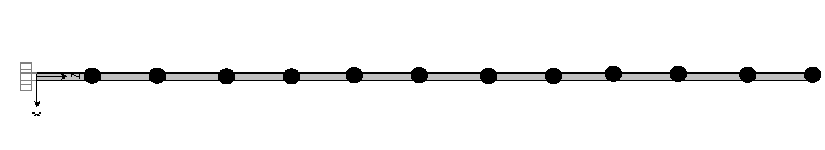
\includegraphics[width=.23\textwidth, height=0.05\textwidth]{originalbeam}}
%\qquad
\subfloat[]{\label{fig:mode1}
%\figurecurrentwidth{mode1}}
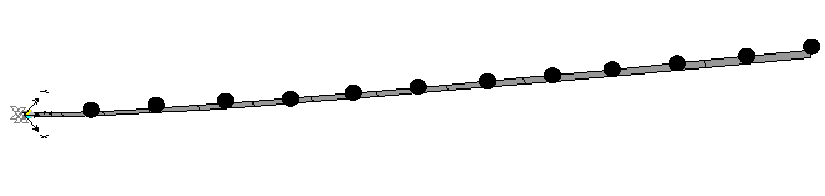
\includegraphics[width=.23\textwidth, height=0.05\textwidth]{mode1}}
\qquad
\subfloat[]{\label{fig:mode2}
%\figurecurrentwidth{mode2}}
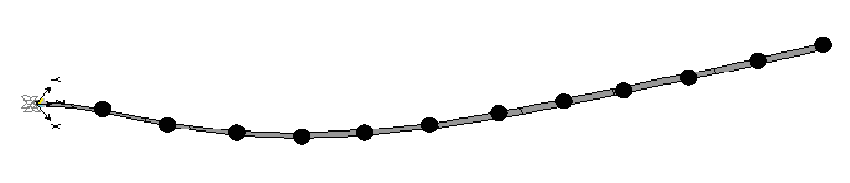
\includegraphics[width=.23\textwidth, height=0.05\textwidth]{mode2}}
%\qquad
\subfloat[]{\label{fig:mode3}
%\figurecurrentwidth{mode3}}
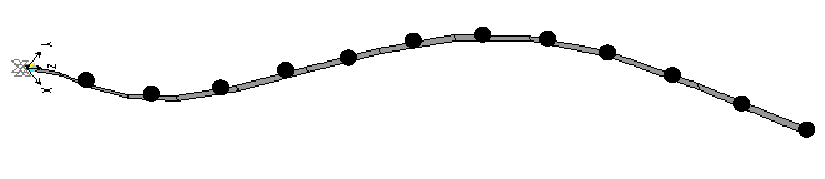
\includegraphics[width=.24\textwidth, height=0.05\textwidth]{mode3}}
%\qquad
%\subfloat[Mode 4 (Freq.=30.8Hz)]{\label{fig:mode4}
%\figurecurrentwidth{mode4}}
%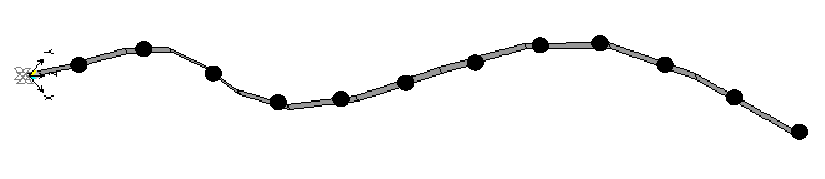
\includegraphics[width=.49\textwidth, height=0.05\textwidth]{mode4}}
\caption{Mode shapes of a typical cantilevered beam (a) Original beam (b)Mode Shape 1 (c) Mode Shape 2(d) Mode Shape 3}
\label{fig:modes}
\end{figure}

It can be seen that mode shape vector \(\mathbf{\Psi_k}\) has an element corresponding to each sensor node. The more number of sensor nodes used, the more elements are contained in \(\mathbf{\Psi_k}\), and more accurately this vibration pattern of the structure is described. Considering example in Fig. \ref{fig:modes}, if we double the number of nodes deployed on the beam, the vibration patterns will be represented with higher granularity. Another important characteristic of mode shape is that elements in \(\mathbf{\Psi_k}\) only represent the relative vibration amplitudes of structure at corresponding sensor nodes. That is, \(\mathbf{\Psi_k}=\zeta \mathbf{\Psi_k}\), where \(\zeta\) is any non-zero real number. This property will be re-visited when we formulate the clustering problem in section \ref{sec:OptimalClustering}.

\subsection{Cluster-based Modal Analysis and Its Energy Consumption}
In this section, we first give an overview of this cluster-based approach and then formulate the energy consumption of cluster-based modal analysis.

In the cluster-based modal analysis, deployed sensor nodes are partitioned into a number of single-hop clusters and each CH performs intra-cluster modal analysis to extract local mode shapes. Since mode shapes of a cluster only contain elements corresponding to the sensor nodes in that cluster, the mode shapes in all the clusters need to be assembled to obtain the mode shapes defined on all the deployed sensor nodes. The whole process is illustrated in Fig. \ref{fig:clusterflow}.

\begin{figure}
	\centering
		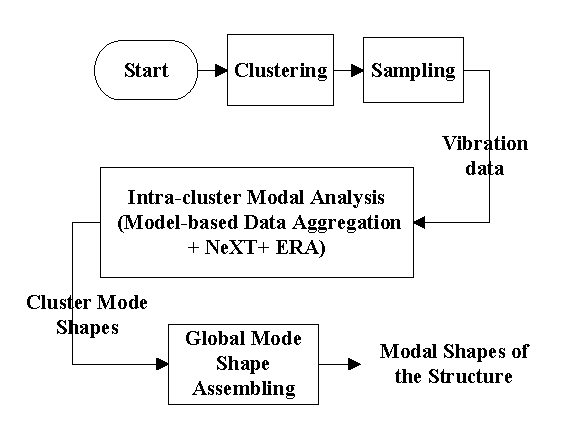
\includegraphics[width=.3\textwidth,height=.2\textwidth]{clusterflow.eps}
	\caption{Overview of cluster-based modal analysis process}
	\label{fig:clusterflow}
\end{figure}

In this paper, the modal parameters are identified using the natural excitation technique (NExT)\cite{james1993natural} in conjunction with the ERA. NexT+ERA is a widely accepted modal analysis approach and can give accurate mode shape estimate using output data-only. 

In each cluster, the NExT is used first to calculate power spectral density (PSD) of the CH and cross spectral density (CSD) between the CH and each of the cluster member. PSD and CSD functions are estimated using:
\begin{equation}
G_{xy}(\omega)=\frac{1}{n_d\cdot n_t}\sum\limits_{i=1}^{n_d}X_i^*(\omega)\cdot Y_i(\omega) \label{eq:next}
\end{equation}
where \(G_{xy}(\omega)\) is the CSD between two vibration signals, \(x(t)\) and \(y(t)\), measured from CH and a cluster member, respectively. \(X(\omega)\) and \(Y(\omega)\) are the Fourier transforms of \(x(t)\) and \(y(t)\), and '*' denotes the complex conjugate. \(n_t\) is time length of each record \(x_i(t)\) or \(y_i(t)\). \(n_d\) is the number of averages mainly for denoising purpose and \(n_d\) practically ranges from 10 to 20. When calculating \(G_{xy}\), consecutive records of \(x_i(t)\)(also \(y_i(t)\)) generally overlap. When \(y(t)\) in Eq. \ref{eq:next} is replace by \(x(t)\), the power spectral density (PSD) of CH is obtained. 

After obtaining CSD and PSD functions, the inverse Fourier transform is implemented and the cross-correlation functions (CCFs) and auto-correlation function (ACF) are obtained.  The ERA uses these functions to build a state space system whereby mode shapes of the structure are identified.

Traditionally, CH collects the raw data from all its cluster members, calculates CSDs and its PSD, and then uses the ERA to identify mode shapes.  However, the model-based data aggregation method proposed by \cite{nagayama2008structural} can be used here to decrease the energy consumption. In this approach, instead of collecting measurements data from cluster members, CH broadcasts its time record of length \(n_t\). On receiving the record, each cluster member calculates its CSD and stores it locally.  This procedure will be repeated \(n_d\) times, until the CSD is according to Eq. \ref{eq:next}. Each cluster member then transmits the first half of the corresponding CCF to the CH.
\begin{comment}
\begin{figure}
	\centering
		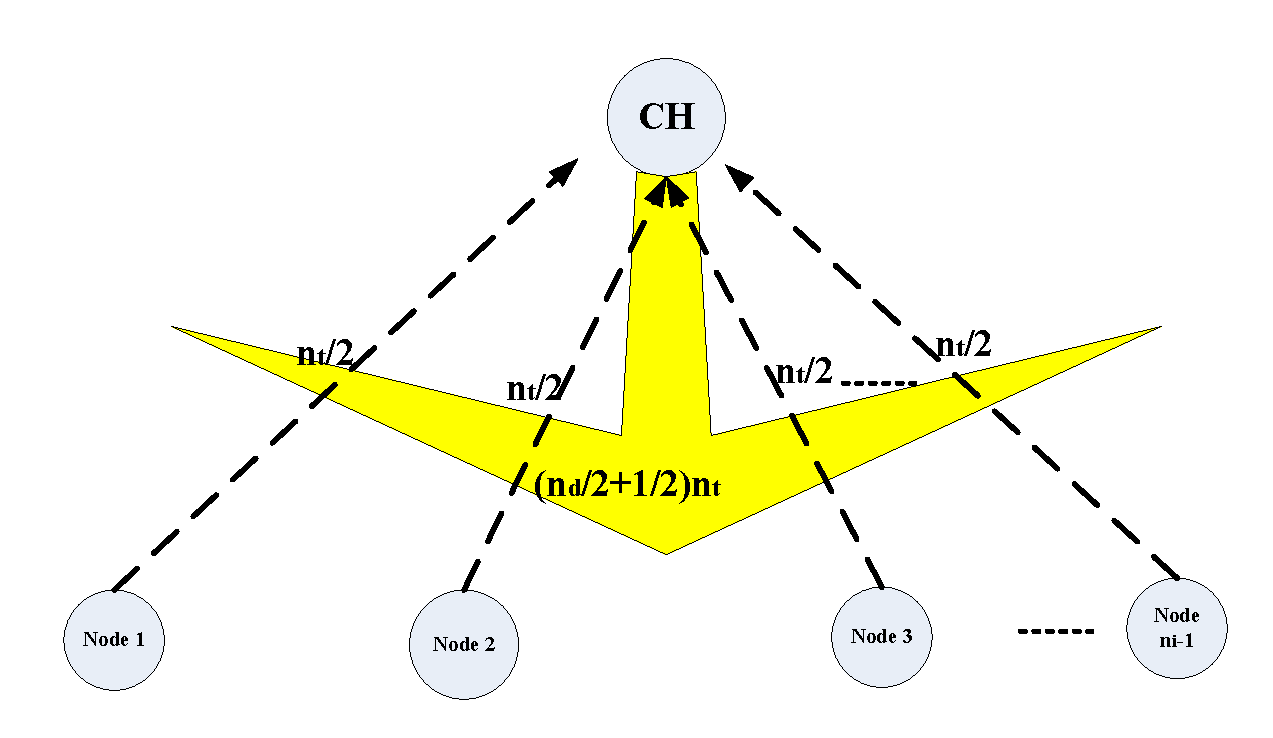
\includegraphics[width=.3\textwidth,height=.18\textwidth]{clusteraggregation.eps}
	\caption{Model-based data aggregation (Assume 50 \% Overlap)}
	\label{fig:clusteraggregation}
\end{figure}
\end{comment}

Based on the discussion above, we can estimate the energy consumption of intra-cluster modal analysis. To obtain the mode shapes of a cluster \(S_i\), the total energy consumption in \(S_i\), denoted as \(cost(S_i)\), can be mainly decomposed into the following three parts: 
\begin{subequations}
\begin{equation}
cost(S_i)=Er_s(S_i)+Er_c(S_i)+Er_a(S_i)
\end{equation}

where \(Er_s(S_i)\), \(Er_c(S_i)\)  and \(Er_a(S_i)\) are the energy consumed in data sampling, intra-cluster wireless communication and computation associated with modal analysis, respectively. 

Assume a cluster \(S_i\) contains a total of \(n_i\) sensor nodes, then sampling cost \(Er_s(S_i)\) is:
\begin{equation}
Er_s(S_i)=n_i\cdot N\cdot e_S
\end{equation}

where \(N\) is the total amount of time history record sampled in each sensor. Assuming 50 \% overlapping,  \(N=(n_d/2+1/2)n_t\). \(e_S\) is the energy for sampling one data. We assume that \(n_d\) , \(n_t\), \(N\) and \(e_S\) are fixed in this paper.  

The intra-cluster wireless communication cost \(Er_c(S_i)\) is:
\begin{align}
Er_c(S_i)=&N\cdot e_T+(n_i-1)N\cdot e_R\nonumber \\
+&(n_i-1)\frac{n_t}{2}(e_T+e_R) \label{eq:energytotal}
\end{align}
where \(e_T\) and \(e_R\) are the energy cost for transmitting and receiving one data, respectively. The first two terms at the right side of Eq. \ref{eq:energytotal} are the energy consumed when CH broadcasts its time history data and when all the cluster members receive the broadcasts, respectively. The last term is the energy consumption when the \((n_i-1)\) cluster members transmit back their correlation functions to the CH.

The computation cost \(Er_a(S_i)\) can be formulated as:
\begin{equation}
Er_a(S_i)=n_i\cdot e_{NExT}+e_{ERA}(n_i)
\end{equation}
\end{subequations}

where \(e_{NExT}\) is the energy consumed when each node implements the NExT (including calculating the CSD/PSD and CCF/ACF) and \(e_{ERA}\) is the energy used in CH when it carries out the ERA for mode shape identification. \(e_{NExT}\) is fixed given  \(n_t\) and \(n_d\). \(e_{ERA}\) is dependent on \(n_i\) and number of mode shape vectors \(p\) to be identified.  Given \(p\), \(e_{ERA}(n_i)\) is not a linear function of \(n_i\) since the ERA involves complex matrix computations including SVD and matrix inversion. This point is demonstrated in Fig. \ref{fig:ERAcomplexity}, where the computation time of our SHM mote to implement the ERA for different cluster sizes is illustrated. The fitting function is also illustrated in the figure. It can be seen that with the increase of \(n_i\), the time consumed, which is the indicator of energy consumption, is quadratically increased.
\begin{figure}
	\centering
		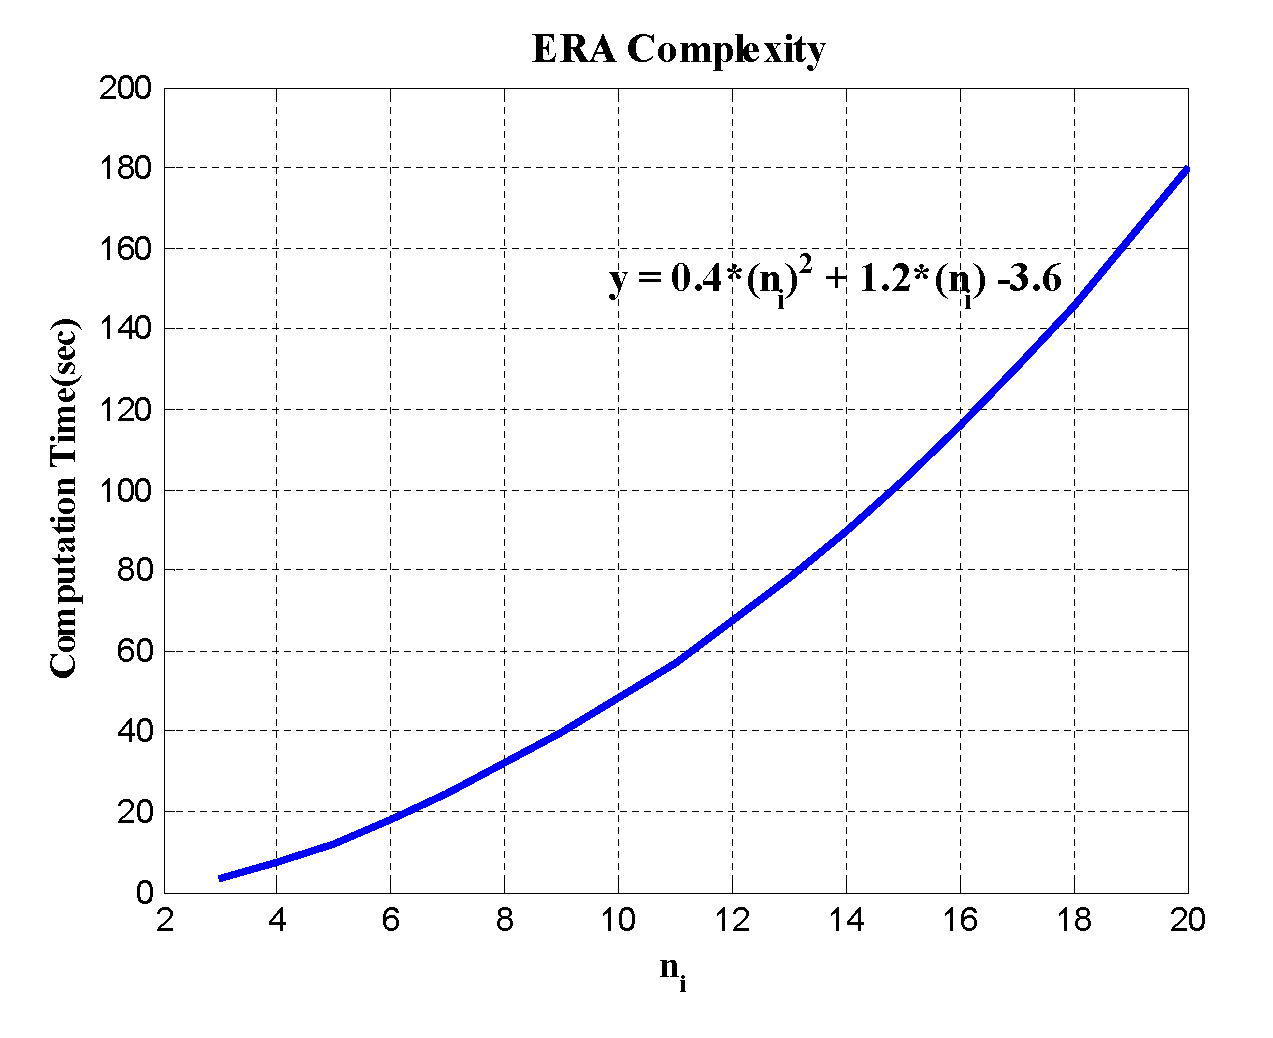
\includegraphics[width=.28\textwidth,height=.20\textwidth]{ERAcomplexity.eps}
	\caption{The complexity of the ERA}
	\label{fig:ERAcomplexity}
\end{figure}

From the equations above, we have \(cost(S_i)=cost(n_i)\), indicating that the energy consumption of a cluster is only associated with the number of sensor nodes in this cluster. It is of interest to see that if possible, whether to generate small-sized clusters or large-sized clusters is more energy efficient.  To find the answer, we assume \(M\) sensor nodes can be partitioned into equal-sized clusters of size \(n\), then the number of clusters \(c = M/n\). The optimal cluster size, denoted as \(n_{opt}\), can be obtained by looking for the \(n\) that minimizes the average energy consumption per node defined as: 

\begin{align}
\label{eq:nooverlap}
Epn(n) = \frac{c\cdot cost(n)}{M} = N(e_S+\beta) + e_{NExT}\\ \nonumber 
+ \frac{N(e_T-\beta)}{n} + \frac{e_{ERA}(n)}{n} 
\end{align}
where \(\beta =e_R+\frac{n_t}{2N}(e_T+e_R)\).

The \(3^{rd}\) term in the right side of the Eq. \ref{eq:nooverlap} indicates that in terms of wireless communication, partitioning sensor network into large-sized clusters is preferred when \(e_T \geq \beta\) while generating small-sized clusters is better if otherwise. The \(4^{th}\) term tells us that small cluster size \(n\) is more energy efficient in terms of computation considering that \(e_{ERA}(n)\) is a quadratic function of \(n\). As a result, there does not exist a rule of thumb for clustering and we have different optimal cluster sizes for different conditions. As an example, some parameters obtained by some real tests of our SHM Mote are listed in Table \ref{tab:Table2}. Based on Table \ref{tab:Table2}, Fig. \ref{fig:MagicNumber2}a shows various optimal cluster sizes, illustrated as red dots in the figure, when the transmission power \(e_T\) is set to be from \(e_T = e_R\) to \(e_T = 5 e_R\). It can be seen that when \(e_T=e_R\), the smaller the cluster size, the better. (Note that the ERA requires that the number of sensor nodes in each cluster should be at least larger than \(p\)). With the increase of \(e_T\), the optimal cluster size is increased but does not go unbounded considering the energy consumption of the ERA for large-sized clusters.

\begin{figure}
	\centering
		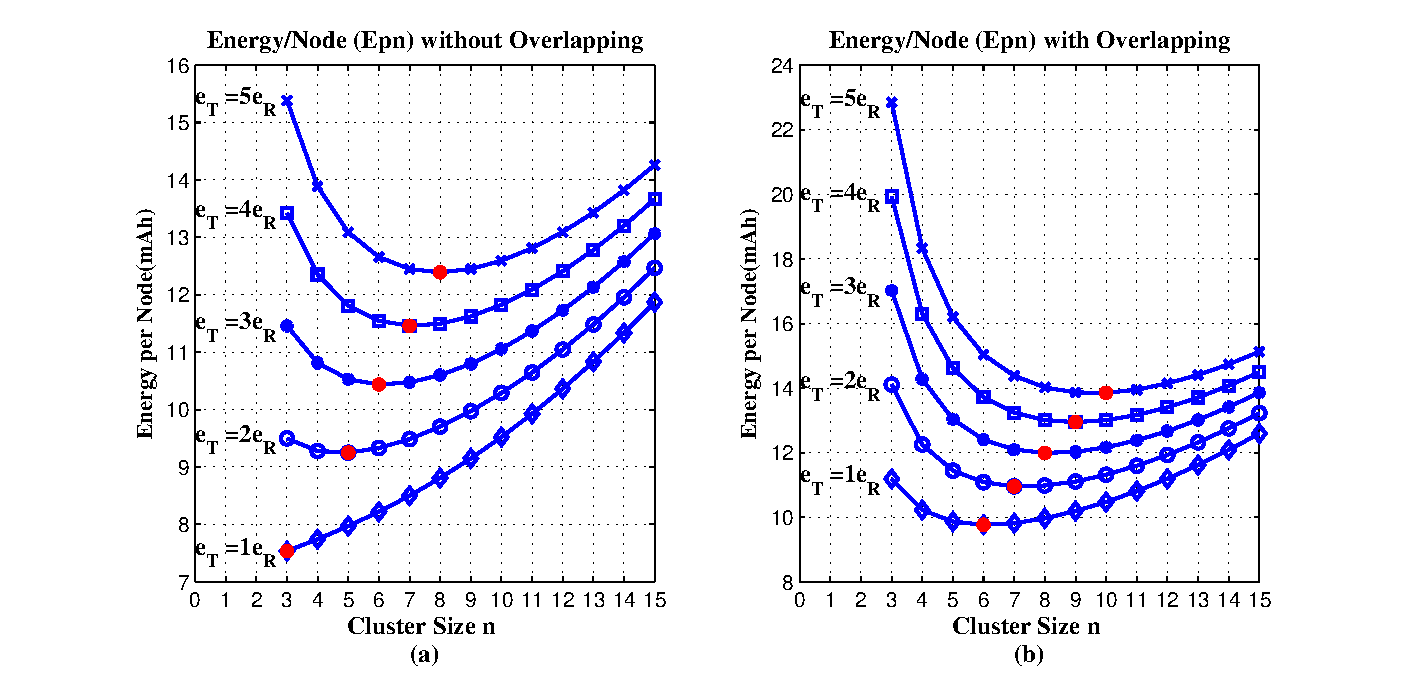
\includegraphics[width=.5\textwidth,height=.25\textwidth]{EnergyPerNode.eps}
	\caption{The optimal cluster sizes in different conditions. (a)No overlapping (b)with overlapping}
	\label{fig:MagicNumber2}
\end{figure}


\begin{table}
	\centering
\begin{tabular}{|c|c|c|c|c|c|c|c|}
\hline
\(N\)&\(p\)&\(n_t\)&\(n_d\)&\(e_S\)&\(e_R\)&\(e_{NExT}\)&\(e_{ERA}\)\\
& & & &(mAh)&(mAh)&(mAh)&(mAh)\\
\hline
     &     &       &       &       &   & &\(0.0417(0.4n_i^3\)\\
10752&3&1024&20&1.1e-4&5e-4&0.5&\(+1.2n_i\)\\
&&&&&&&-3.6)\\
\hline
\end{tabular}
	\caption{Parameters used in Fig. \ref{fig:MagicNumber2}}
	\label{tab:Table2}
\end{table}

Clustering using minimum dominating set \cite{wan2004distributed} or maximum independent set 
\cite{banerjee2001clustering} cannot be directly applied to solve our clustering problem since they mainly aim to find as small number of clusters as possible. Also, in the discussion so far, we assume that no overlapping nodes exist in the clusters. However, we will show in the following section that a necessary condition for cluster-based modal analysis is that all the generated clusters must be connected through the overlapping nodes. This requirement further increases the difficulty of the clustering problem.

\subsection{Determination of Global Mode Shapes through Mode Shape Assembling}
After the mode shapes in all clusters have been identified, they need to be stitched together to obtain mode shapes defined on all of deployed sensor nodes. 

However, since mode shape vectors identified in a cluster only represent the relative vibration amplitudes at cluster sensor nodes, mode shapes of different clusters may not be able to be assembled together. This can be demonstrated in Fig. \ref{fig:TwoTypesClustering}a, where the deployed 12 sensor nodes in Fig. \ref{fig:modes} are partitioned into three clusters to identify the \(3^{rd}\) mode shape.  Although the mode shape of each cluster is correctly identified, we still cannot obtain the mode shapes for the whole structure. The key to solve this problem is overlapping.  We must ensure that each cluster has at least one node which also belongs to another cluster and all the clusters are connected through the overlapping nodes (a more formal definition will be given in the next section).  For example, in Fig. \ref{fig:TwoTypesClustering}\((b)\), mode shapes identified in each of the three clusters can be assembled together with the help of the overlapping nodes \(5\) and \(9\). This requirement of overlapping must be satisfied when formulating the problem of optimal clustering.

\begin{figure}
\centering
\subfloat[]{\label{fig:NonOverlapClusterBeam}
%\figurecurrentwidth{originalbeam}}
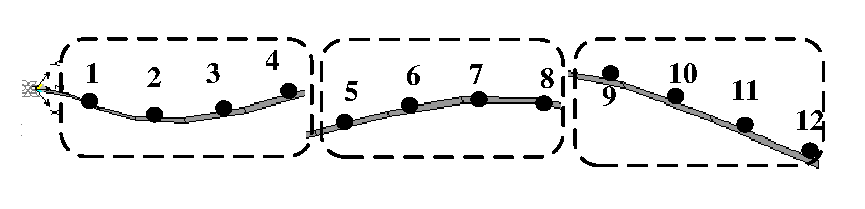
\includegraphics[width=.25\textwidth, height=0.08\textwidth]{NonOverlapClusterBeam}}
%\qquad
\subfloat[]{\label{fig:OverlapClusterBeam}
%\figurecurrentwidth{mode1}}
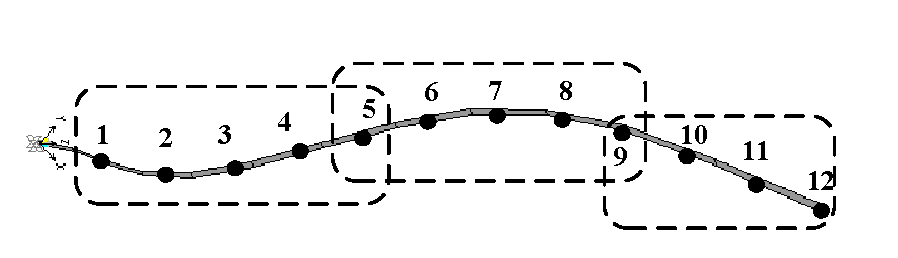
\includegraphics[width=.25\textwidth, height=0.08\textwidth]{OverlapClusterBeam}}
\caption{Mode shape assembling when (a) clusters do not overlap (b) clusters overlap}
\label{fig:TwoTypesClustering}
\end{figure}

It is obvious that overlapping will affect the overall energy consumption and consequently, the optimal cluster size \(n_{opt}\) will be different from that when no overlapping is considered.  By defining the number of overlapping nodes as \(n_o = \sum\limits_{i=1}^c\left|S_i\right| - M\), and still assume these \(M\) sensor nodes are partitioned into equal-sized clusters of size \(n\), then the energy consumption per node becomes

\begin{align}
\label{eq:MagicNumberOverlapping}
Epn'(n) = \frac{(M+n_o)/n \cdot cost(n)- n_o \cdot N \cdot e_S}{M}\\ \nonumber
=\frac{cost(n)}{n}  + \frac{n_o}{M} \cdot \kappa
\end{align}

where \(\kappa = N \cdot \beta + e_{NExT}+ \frac{N(e_T-\beta)}{n} + \frac{e_{ERA}(n)}{n}\).  Considering the fact that unnecessary overlapping will cause extra energy consumption and the number of overlapping nodes should be kept as small as possible, we require that \(n_o \geq \frac{M+n_o}{n} -1\). Therefore,

\begin{equation}
\label{eq:MagicNumberOverlapping2}
Epn'(n) \geq \frac{cost(n)}{n}+ \frac{1-n/M}{n-1}\kappa
\end{equation}

The right side of Eq. \ref{eq:MagicNumberOverlapping2} essentially provides a lower bound of energy consumption that clustering can achieve when the overlapping constraint is considered. The optimal cluster size \(n_{opt}\) can be calculated by minimizing \(n\) in Eq. \ref{eq:MagicNumberOverlapping2}.  For example, the \(n_{opt}\) for the parameters listed in Table \ref{tab:Table2} are illustrated in Fig. \ref{fig:MagicNumber2}b. 

By comparing Fig.\ref{fig:MagicNumber2}a with Fig.\ref{fig:MagicNumber2}b, it also can be easily seen that optimal cluster size is larger when overlapping constraint is considered. Clustering which generates small-sized clusters may not be energy efficient since a large number of overlapping nodes can cause extra energy consumption in terms of communication and computation. 

Also should be noted is that the optimal cluster size \(n_{opt}\), either obtained by Eq. \ref{eq:nooverlap} or by Eq. \ref{eq:MagicNumberOverlapping2}, is not affected by actual network topology. In a dense network, it is more possible to achieve the obtained optimal cluster size and therefore, the total energy will be lower than a sparse network.

We do not consider the inter-cluster communication in this paper simply because delivering obtained mode shapes requires significantly less energy than other processes.

\subsection{Optimal Clustering}
\label{sec:OptimalClustering}
In this section, we will formulate the optimal clustering problem.  The objective of clustering is that the generated clusters can minimize the energy consumption of overall modal analysis. Clustering also has to satisfy the following constraints (1) each sensor node belongs to at least one of the generated clusters, (2) sensor nodes in each cluster is within a single communication range to its CH, (3) number of sensor nodes in each cluster is larger than \(p\) (\(p\):the number of mode shape vectors to be identified) (4) all the clusters are connected together through the overlapping nodes. More formally, problem is formulated as follows:
Given a sensor network \(G=(V,E)\), find a clustering scheme that can cluster these \(V\) sensor nodes into a set of clusters, denoted as \(C=\{S_1, S_2, S_3, \cdots\}\), subject to the following constraints:
\begin{enumerate}
	\item \( \bigcup\limits_{S_i \in C} = V\)
	\item Let the sub-graph for \(S_i\) is \(G(S_i,E_i)\), where \(E_i \subseteq E\). Then \(\forall S_i \in C, \exists s_i \in S_i\), such that there is an edge \(a_{ij} \in E_i\) between \(s_i\) and any other \(s_j \in S_i (s_i \neq s_j)\) 
	\item \(\forall S_i \in C, \left|S_i\right|\geq p\)
	\item \( \forall S_i, \exists S_j \in C, (i \neq j), S_i \bigcap S_j \neq \emptyset\)
	\item \(\forall C' \subseteq C, (\bigcup\limits_{S_i \in C'} S_i)\bigcap (\bigcup\limits_{S_j \in C-C'} S_j) \neq \emptyset \)
\end{enumerate}
Objective:
\begin{itemize}
\item Minimize \(\sum\limits_{S_i \in C} cost(S_i)\)
\end{itemize}

The first constraint is set because we wish to find the mode shapes defined on all the deployed sensor nodes. The second constraint is to ensure only single-hop clusters are generated. Constraint 3 is required by the ERA algorithm. Constraints 4 and 5 are used to describe that generated clusters are overlapping and connected. 

The above clustering problem is an optimization problem. We will prove that the decision version of the problem is NP complete which is defined as: \emph{given a threshold \(k\) , does there exist a cluster set \(C=\{S_1, S_2, S_3, \cdots\}\), which satisfy all the constraints above and whose total energy cost \(\sum\limits_{S_i \in C} cost(S_i)\) is equal of smaller than \(k\)?}.

\begin{theorem}
The decision version of our clustering problem is NP-complete.
\end{theorem}

\begin{proof}
It is easy to find out this clustering problem is NP.  Given a cluster set \(C\), all the constraints above, include constraints 4 and 5 can be checked in a polynomial time. The detailed proof of this part is omitted for brevity.

We show this decision version of the clustering problem is NP-hard by reducing the set cover problem to it. The set cover problem is defined as follows.

\begin{flushleft}
\textbf{Given:}
\end{flushleft}
\begin{enumerate}
\item A universe \(V'\)
\item A set of \(S'=\{S'_1, S'_2, ...\}\subseteq V'\)
\item The cost function for each subset \(S'_i\in S'\): \(cost'(S'_i)\) 
\item A number \(k'\)
\end{enumerate}
\textbf{Find: }
If there is a subset \(C'\subseteq S'\) which satisfies
\begin{enumerate}
\item \( \bigcup\limits_{S'_i \in C'} S'_i =V'\)
\item \( \sum\limits_{S'_i \in C'} cost'(S'_i) \leq k'\)
\end{enumerate}

To reduce the set cover problem to the clustering problem, we construct a sensor network \(G=(V, E)\) from the inputs of set cover problem in the following way:
The vertices \(V =V'\bigcup X\) , where \(X = \{x_1,x_2,...x_p\}\)  is a set of \(p\) virtual nodes. 
To construct the edges \(E\), for each \(S'_i\in S'\) , we first choose an arbitrary  node \(s'_i\in S'_i\), then we add an edge between \(s'_i\) and any other node \(s'_j \in S'_i (s'_j\neq s'_i)\). We also add an edge between \(s'_i\) and any virtual node in \(X\). 
The cost function in the clustering problem \(cost(\cdot) = cost'(\cdot)\). We also define that by adding/deleting any virtual node \(x\) to/from any group will not affect the cost function. The energy threshold \(k=k'\). 

With this transformation, it can be easily proved that 1) Assume \(C'=\{S'_1, S'_2, ...\}\)is a solution to the set cover problem, then \(C=\{S_1, S_2, ...\}\)  is a solution to the clustering problem, where \(S_i = S'_i \bigcup X\). 2) Assume \(G =(V,E)\) is constructed from the set cover problem and we have a solution \(C=\{S_1, S_2, ...\}\) to the clustering problem, then \(C'=\{S'_1, S'_2, ...\}\) is a solution to the set cover problem, where \(S'_i=S_i - X\). The detailed proof is omitted for brevity. 
\end{proof}
By reducing the NP-complete set problem to our clustering problem, we have demonstrated that the decision version of our problem is NP-complete. Obviously, the original clustering problem is also NP-Complete.
\section{Proposed Methods for Energy Efficient Clustering}
\label{sec:solution}
\subsection{Two Centralized Algorithms}
\label{sec:centralizedsolution}
Two centralized algorithms are proposed to solve our clustering problem. These two algorithms use the similar idea of the greedy algorithm for the set cover problem but adopt different approaches to handle the extra constraints of clustering. In both of the algorithms, a set of candidate single-hop clusters is first established given the network  \(G =(V,E)\). Then the most cost-effective cluster is selected from this set, one at a time, until all the sensor nodes in \(V\) have been covered.  

In the first algorithm, to find a candidate cluster set \(U\), we first calculate the optimal cluster size \(n_{opt}\) according to Eq. \ref{eq:MagicNumberOverlapping2}. Then based on \(n_{opt}\), one-hop neighbors of each node in \(V\) are partitioned. For each node \(s_i \in V\), assume the one-hop neighbor set is \(Ne_{s_i}\), if \( \left|Ne_{s_i}\right| \geq n_{opt}-1\), then each cluster in the cluster set contains a common element \(s_i\) and the remaining elements are the combinations of nodes in \(Ne_{s_i}\) with the length of \(n_{opt}-1\). When \(\left|Ne_{s_i}\right| < n_{opt} -1\), \(C_i =\{s_i\} \bigcup Ne_{s_i}\). Note that we assume the network is dense enough such that each sensor node has at least \(p\) one-hop neighbors. The obtained cluster sets for all the nodes in \(V\) are combined together to obtain the candidate cluster set \(U\).

The algorithm then selects the most cost-effective cluster \(S_i \in U\), one at a time, until all the sensor nodes in \(V\) have been covered. The cost effectiveness, denoted as \(\lambda\), is defined as \(\lambda = \frac{1}{\left|S_i\cup C_a\right| - \left|C_a\right|}\), where \(C_a\) represents the set of nodes covered so far. When selecting the most cost-effective cluster, we choose from the clusters in \(U\) which overlap with \(C_a\). This strategy can ensure that all the selected sensor nodes will be connected through the overlapping nodes.  If more than one candidate clusters which overlap with \(C_a\) have the same \(\lambda\), the one which maximizes the total degrees of the remaining un-covered nodes (i.e. \(U- S_i\bigcup C_a\)) will be chosen. It can be seen that this algorithm divides the sensor nodes in \(V\) into as many single-hop clusters of size \(n_{opt}\) as possible while keeps the number of overlapping nodes into minimums (from \(\lambda = \frac{1}{\left|S_i\cup C_a\right| - \left|C_a\right|}\), penalty is given to cluster having large number of overlapping nodes with \(C_a\)). Both of these two points are of importance to minimize the overall energy cost. The algorithm is shown as Algorithm \ref{algo:greedy1}.

The second algorithm uses different strategy to handle overlapping.  First, the optimal cluster size \(n_{opt}\) is calculated based on Eq. \ref{eq:MagicNumberOverlapping} without considering overlapping constraint. When selecting the most cost effective cluster, it is chosen from all the candidate clusters in \(U\). Since the overlapping constraint is not considered when selecting cluster, after all the sensor nodes in \(V\) have been covered, the algorithm will test if all the clusters are connected through the overlapping nodes and add extra clusters to connect them if necessary. The basic idea is to identify all the isolated cluster groups and then find clusters to connect them. The detailed description is omitted for brevity. This algorithm is shown as Algorithm \ref{algo:greedy2}. 

\begin{comment}
To achieve this, all the isolated cluster groups (ICGs) from the obtained clusters are identified . Clusters within an ICG are connected through overlapping nodes but do not overlap with other ICGs. Each ICG is then represented as a vertex in a graph \(G_{ICG}\). There is an edge between two vertices in \(G_{ICG}\) if there exist two nodes, each within a ICG corresponding to one of the two vertices, are within the communication range of each other. Then the minimum spanning tree (MST) is found that can connect all the vertices in \(G_{ICG}\). For each edge in the MST, an extra cluster is established in which the two sensor nodes associated with the edge are included. If \(p \geq 2\), then additional nodes should also be added to satisfy the constraint 3 of the optimal clustering problem. This algorithm is shown as Algorithm \ref{algo:greedy2}.
\end{comment}

\begin{algorithm}
\begin{algorithmic}[1]
\REQUIRE \(G=(V, E)\) and parameters listed in Table. \ref{tab:Table2}
\STATE find \(n_{opt}\) which minimizes Eq. \ref{eq:MagicNumberOverlapping}
	\STATE \(U\gets \emptyset\) \(C_a\gets \emptyset\)
	\FORALL {\(n_i\in V\)}
		\STATE \(S_i\gets \emptyset\)
		\FORALL {one hop neighbor \(n_j\) of \(n_i\)}
			\STATE \(S_i = S_i \bigcup \{n_j\}\)
		\ENDFOR
		\STATE construct a cluster set \(C_i\) whose elements are the combinations taken of the nodes in \(S_i\) of length \(n_{opt} - 1\).
		\STATE \(U=U\bigcup C_i\)
	\ENDFOR
	 	\REPEAT
	 \STATE \(C_{cand} =\) all the clusters in \(U\) which overlap with \(C_a\)
		\STATE find a cluster \(S_i\) in \(C_{cand}\) with the smallest \(\frac{1}{\left|S_i\cup C_a\right| - \left|C_a\right|}\)
		\STATE \(C_a=C_a\bigcup S_i\)	
		\UNTIL {\(C_a\) covers \(V\)}
	\ENSURE \(C_a\)
\end{algorithmic}
\caption{Centralized algorithm 1}
\label{algo:greedy1}
\end{algorithm}

\begin{algorithm}
\begin{algorithmic}[1]
\REQUIRE \(G=(V, E)\) and parameters listed in Table. \ref{tab:Table2}
\STATE find \(n_{opt}\) which minimizes Eq. \ref{eq:nooverlap}
  \STATE The same with the 2 to 16 lines of Algorithm \ref{algo:greedy1}
  	\REPEAT
		\STATE find a cluster \(S_i\) in \(U\) with the smallest \(\frac{1}{\left|S_i\cup C_a\right| - \left|C_a\right|}\)
		\STATE \(C_a=C_a\bigcup S_i\)
	\UNTIL {\(C_a\) covers \(V\)}
	\STATE Identify Isolated cluster groups (ICGs) in \(C_a\)
	\STATE Construct a graph \(G_{ICG}=(V_{ICG}, E_{ICG})\):
 \STATE Run MST algorithm on \(G_{ICG}\) and get \(T\)
	\FORALL {edges in \(T\)}
		\STATE Create an extra cluster \(C_e\) and add it to \(C_a\)
	\ENDFOR
	\ENSURE \(C_a\)
\end{algorithmic}
\caption{Centralized algorithm 2}
\label{algo:greedy2}
\end{algorithm}

\begin{comment}
We will use a simple example to demonstrate the two algorithms above. Fig. \ref{fig:AlgorithmExampleNew}(a) plots a graph consisting of a total of 12 nodes. Assume we use the parameters associated with energy listed in Table 1 and the optimal \(n_{opt}\)=4. For simplicity, we also assume that the \(cond(S_i)<\gamma\) if \(\left|S_i\right| \geq p = 3\). Using the generated candidate cluster sets, 4 clusters are obtained using the first algorithm and illustrated in Fig. \ref{fig:AlgorithmExampleNew}(b). Note that all these 4 clusters are connected through the overlapping nodes. Using the second algorithm, a total of 3 clusters are generated after all the 12 nodes have been covered (see Fig. \ref{fig:AlgorithmExampleNew}(c)). However, these clusters do not overlap. Therefore, two extra clusters are generated to connect these isolated clusters. Note that since the minimum number of vibration patterns is 3, each extra cluster contains three nodes. The final clustering result of the second algorithm is shown in Fig. \ref{fig:AlgorithmExampleNew}(d). The total amount of energy using the generated clusters from the first algorithm is about \(0.88\) times of that of the second algorithm. 

\begin{figure}
	\centering
		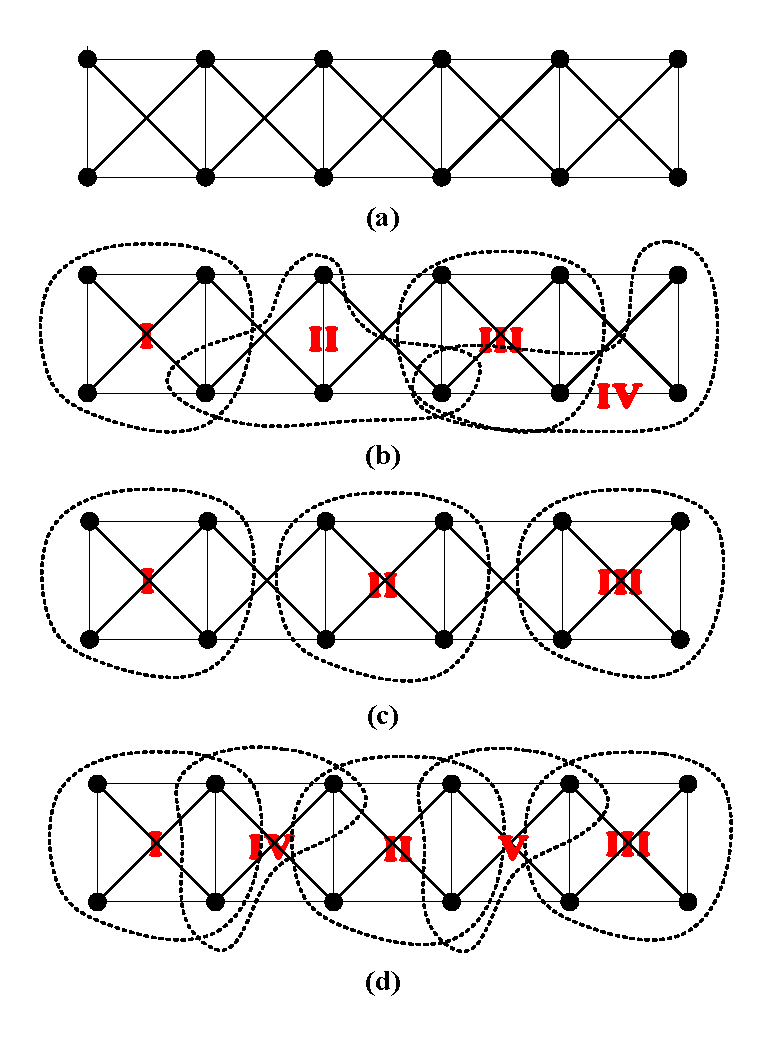
\includegraphics[width=.3\textwidth,height=.35\textwidth]{AlgorithmExampleNew.eps}
	\caption{Example of using the Proposed Algorithms (a) Graph G(V,E), (b) The 4 Clusters Generated from the \(1^{st}\) Algorithm (c) Isolated Cluster Groups from the \(2^{nd}\) Algorithm (e) Final 5 Clusters from the \(2^{nd}\) Algorithm}
	\label{fig:AlgorithmExampleNew}
\end{figure}
\end{comment}

\subsection{A Distributed Algorithm}
Based on our first centralized algorithm, we propose a distributed solution. In this solution, each node only needs its one-hop neighbors information and communicates only with its one-hop neighbors. The clustering will start at a single controller node which usually is the sink node of the network.

Similar to Algorithm \ref{algo:greedy1}, each newly created cluster will be connected to at least one of the existing clusters. In the distributed algorithm, each node will maintain two lists of neighbors: unclustered and clustered. The lists will be sorted according to each neighbor's own number of unclustered neighbors. The nodes with fewer unclustered neighbors will do clustering or join other clusters first. This is done by assigning each node's execution of the algorithm to a specific time slot.

Each node has only three roles during clustering: unclustered, CM (cluster member) and CH. We illustrate the pseudo code based on the three roles in Algorithm \ref{algo:selectionsender}.

\begin{algorithm}
\begin{algorithmic}[1]
\REQUIRE \(n_{opt}\), \(p\), unclustered neighbors \(un\), clustered neighbors \(cn\) (\(un\) and \(cn\) are both sorted in increasing order according to the number of unclustered neighbors)
\IF {self is unclustered}
	\STATE Self becomes CH
\ENDIF
\IF {self is CH}
	\STATE Select one node from \(cn\) as its member
	\IF {\(size(un)\geq n_{opt}\)}
		\STATE Construct the cluster as size of \(n_{opt}\) by selecting first \(n_{opt}\) nodes from \(un\) as CM
	\ELSIF{\(n_{opt}>size(un)\geq p\)}
		\STATE Construct a cluster by selecting all nodes in \(un\) as CM
	\ELSE
		\STATE First construct a cluster by selecting all nodes in \(un\) as CM then select more nodes from \(cn\) as CM until \(cluster\_ size=p\)
	\ENDIF
\ELSIF {self is CM}
	\STATE Broadcast a message to all neighbors saying the status is currently CM.
\ENDIF
\STATE \(an=merge(un, cn)\)
\FORALL {\(n\in an\) that haven't been assigned a time slot}
	\STATE Assign time slot \(t[i]\) to \(n\) where \(i\) is the index of \(n\) in \(an\)
\ENDFOR
\end{algorithmic}
\caption{Distributed algorithm}
\label{algo:selectionsender}
\end{algorithm}

Each node will not execute the algorithm until the start of its own time slot. The input \(p\) is the minimum cluster size constraint and \(n_{opt}\) is the calculated optimal cluster size. Once a CH decides to choose certain node as CM, it will send a message \(req_{ch}\) and the corresponding CM will send \(acpt_{ch}\) to acknowledge the selection. After the execution of the algorithm on a node, an unclustered node will become CH. At the end of the algorithm, each node will merge all its neighbors into one sorted list and assign time slots. The duration of the time slot is large enough so that a CH can perform the selection. \(t[i]\) is the \(i^{th}\) time slot from the end of the current time slot. It can be easily seen that the generated clusters from the distributed algorithm can satisfy all the constraints.

\begin{comment}
Informally, it can be easily shown that the distributed algorithm is correct as the solution it produces will satisfy all the constraints:
\begin{itemize}
\item Since all nodes will be given a time slot to do run the algorithm, the clusters will eventually cover the whole network.
\item The clustering starts at the controller node and all the later CHs will first select a CM from its \(cn\). Therefore, all the clusters will be connected.
\item CH only selects CM within its one-hop neighbors, and the CHs will not remove its role as CH so all clusters will be one-hop.
\item For each CH, it will ensure the cluster size is at least \(p\) by selecting additional CM until the cluster size reaches either \(p\) or \(n_{opt}\).
\end{itemize}
\end{comment}
\section{Performance Evaluation}
\label{sec:PerformanceEvaluation}
\subsection{Simulation}
We first use simulation data to demonstrate the effectiveness of our cluster-based modal analysis approach and the clustering algorithms. We fix all associated parameters except two: the network topology and the transmission power \(e_T\). Although in some circumstances, these two factors are correlated, they are independently considered in this simulation. A total of 40 sensor nodes are randomly deployed starting from a relatively sparse wireless sensor network with network degree, defined using the node with the minimum degree in the network, is 3. Under this network degree, we considered energy consumptions when the transmission power \(e_T\) is changing from \(5e-4\) to \(2.5e-3\), with the interval of \(5e-4\).  The energy consumption of the following four approaches are considered:(1) the traditional approach when all the raw data are streamed back to a sink node, (2) the cluster-based modal analysis with clusters generated from the \(1^{st}\) centralized algorithm, (3) from the \(2^{nd}\) centralized algorithm and (4) from the distributed algorithm. In the first approach, the sink node is chosen to be the node whose short path tree (SPT) is the shortest among all the other nodes. Also, no computation energy is included in this approach. A total of 500 simulations are performed and the average energy consumption of each approach is calculated. The above procedure is repeated when the network degree is changed to be 4 and 5.

The parameters associated with the simulation are listed in Table \ref{tab:Table2} and the simulation results are shown in Fig. \ref{fig:Simulation2}. It can be seen that for the first traditional approach, the total energy is linearly increased with the increase of \(e_T\) and the slope is the length of the SPT rooted at the sink node.  The cluster-based approach, either using clusters generated from centralized or distributed algorithms, is much more energy efficient compared with the traditional approach. This conclusion is more evident when the transmission power \(e_T\) is large. When \(e_T = 2.5e-3\), the energy consumption of the cluster-based approach is about one fifth of the traditional approach.  For the cluster-based approach, it seems that using clusters generated from the \(1^{st}\) centralized algorithm and from the distributed algorithm are slightly better than the \(2^{nd}\) centralized algorithm. 

\begin{figure}
	\centering
		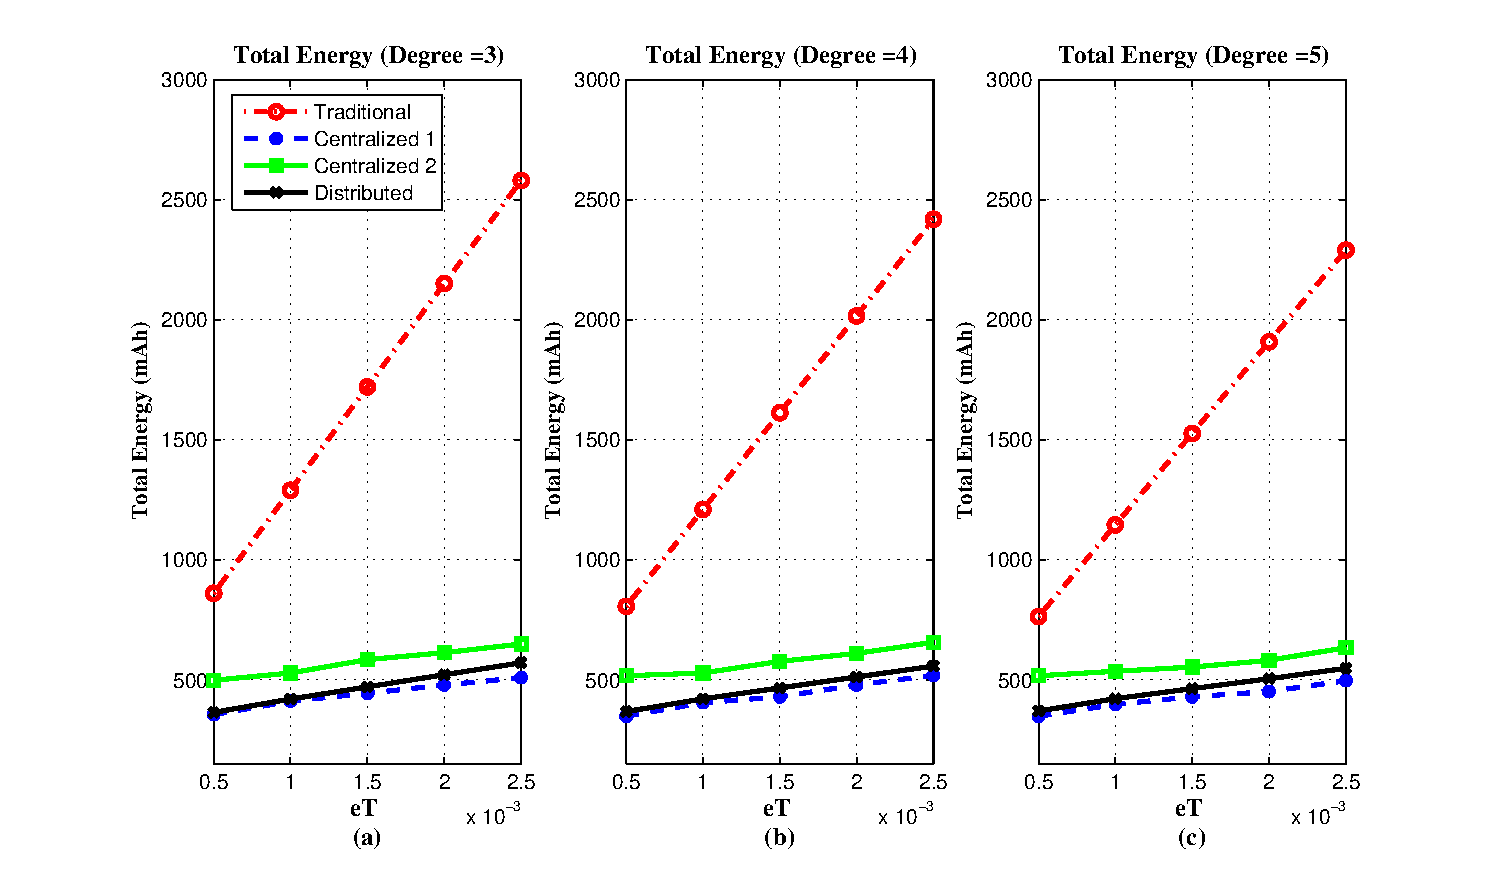
\includegraphics[width=.40\textwidth,height=.25\textwidth]{Simulation2.eps}
	\caption{The total energy in different scenarios. (a)Network Degree=3 (b)Network Degree=4 (c) Network Degree=5}
	\label{fig:Simulation2}
\end{figure}

To further demonstrate the importance of using optimal cluster size, we illustrate in Fig. 
\ref{fig:SimOptNumber} the energy consumption when the \(1^{st}\) algorithm chooses three different cluster sizes: \(n_{opt}-1\), \(n_{opt}\) and \(n_{opt}+1\). It can be seen that compared with other cluster sizes, clustering using designed optimal cluster size can achieve lower energy consumption. 

\begin{figure}
	\centering
		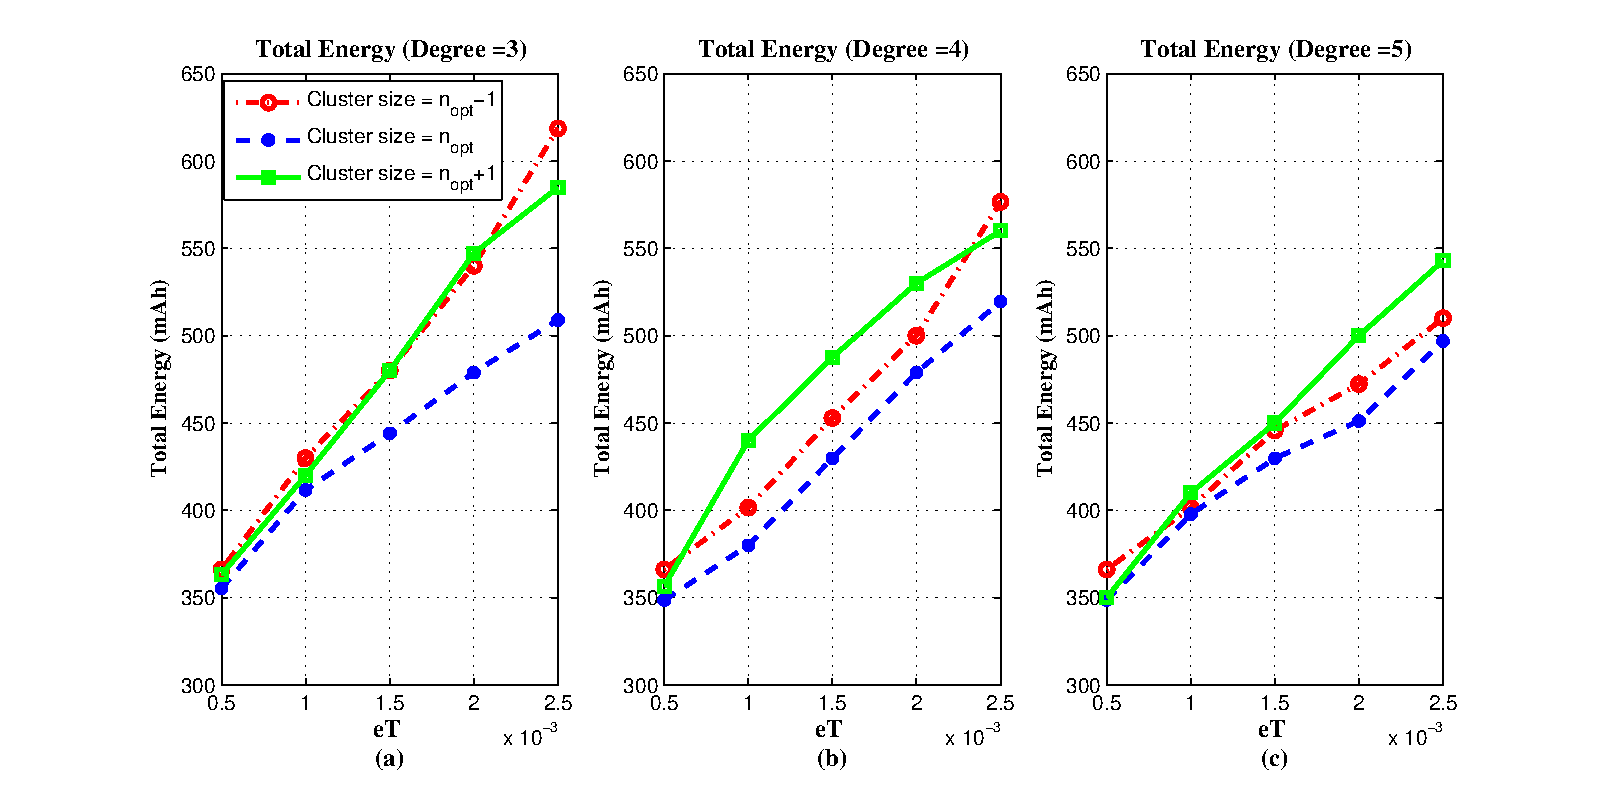
\includegraphics[width=.49\textwidth,height=.25\textwidth]{SimOptNumber.eps}
	\caption{The energy consumption using different cluster sizes. (a)Network Degree=3 (b)Network Degree=4 (c) Network Degree=5}
	\label{fig:SimOptNumber}
\end{figure}

\subsection{Implementation}
We have tested our cluster-based modal analysis approach through a real implementation. The wireless sensor nodes adopted are called SHM Mote and are particularly developed for general SHM applications (see Fig.\ref{fig:SHMMote}). A SHM Mote includes an Intel Imote2, a sensor board, an external 32Mb non-volatile memory chip, an AM radio receiver for synchronized sensing, and a RF amplifier. 

\begin{figure}
\centering
\subfloat[SHM Mote]{\label{fig:SHMMote}
%\figurecurrentwidth{originalbeam}}
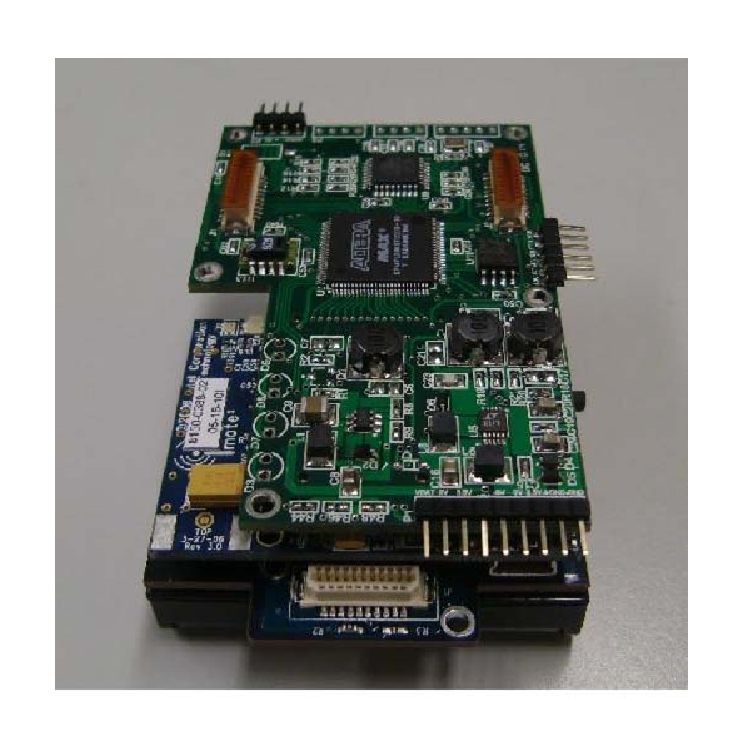
\includegraphics[width=.15\textwidth, height=0.2\textwidth]{SHMMote.eps}}
%\qquad
\subfloat[Testing structure]{\label{fig:TestStructure}
%\figurecurrentwidth{mode1}}
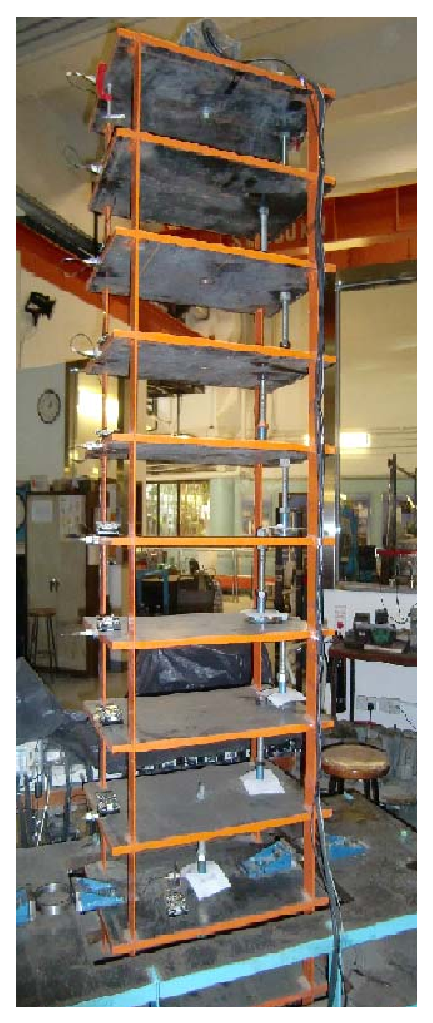
\includegraphics[width=.15\textwidth, height=0.3\textwidth]{TestStructure.eps}}
\subfloat[Network topology]{\label{fig:Testbedtopology}
%\figurecurrentwidth{originalbeam}}
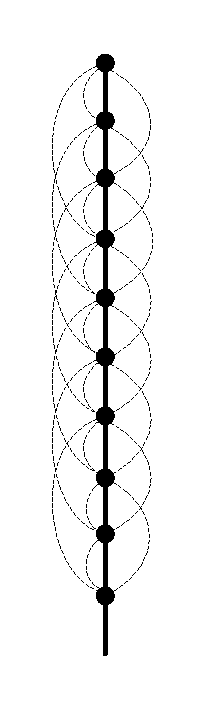
\includegraphics[width=.11\textwidth, height=0.32\textwidth]{Testbedtopology.eps}}
\caption{SHM Mote and testing structure}
\label{fig:SHMMOTEandTestStructure}
\end{figure}

Fig. \ref{fig:SHMMote} shows the setting of the lab test. The test building has 10 floors, at each floor, a Mote is deployed to monitor the structure's horizontal accelerations. We adjust the transmission power to be \(e_T =1e-5\) in this test after a few tests on link-quality. Under this transmission power, the topology of the network along with the simplified structure are illustrated in Fig. \ref{fig:TestStructure}. We use a gateway node which is connected a computer for the control purpose, while this gateway can be removed in future implementation. The SHM Motes run modified TinyOS and are configured to sample the accelerometers in a synchronized manner at frequency of 512Hz. Under the command of gateway, each Mote starts collecting \(N = 10752\) data samples synchronously.  The cluster information is calculated by the \(1^{st}\) centralized algorithm run in the computer and then is feed to each node through wireless link. In this implementation, the optimal cluster size is \(n_{opt}=7\) and these ten sensor nodes are partitioned into 2 clusters as illustrated in Fig. \ref{fig:Testbedtopology}. Once each node has this information, the cluster-based modal analysis is implemented in each cluster, one cluster at a time, to identify the first three mode shapes of the structure.  The obtained mode shapes of each cluster are then transmitted back to the gateway and are assembled.  For comparison, traditional approach is also used in which all measured data are transmitted the gateway where the ERA using all the measurement data to identify the mode shapes of the whole structure.

Fig. \ref{fig:TestResults} illustrates the identified mode shapes by the traditional centralized modal analysis and by our cluster-based modal analysis. It can be seen that using cluster-based modal analysis, the mode shapes can be identified without losing much of the accuracy. Moreover, we tested that the energy communication cost is decreased from \(259mAh\) to \(152mAh\). 

\begin{figure}
\centering
\subfloat[Clustering using algorithm1]{\label{fig:Testbedcluster}
%\figurecurrentwidth{originalbeam}}
\includegraphics[width=.11\textwidth, height=0.32\textwidth]{Testbedclustering.eps}}
\subfloat[Mode shapes]{\label{fig:TestResults}
%\figurecurrentwidth{originalbeam}}
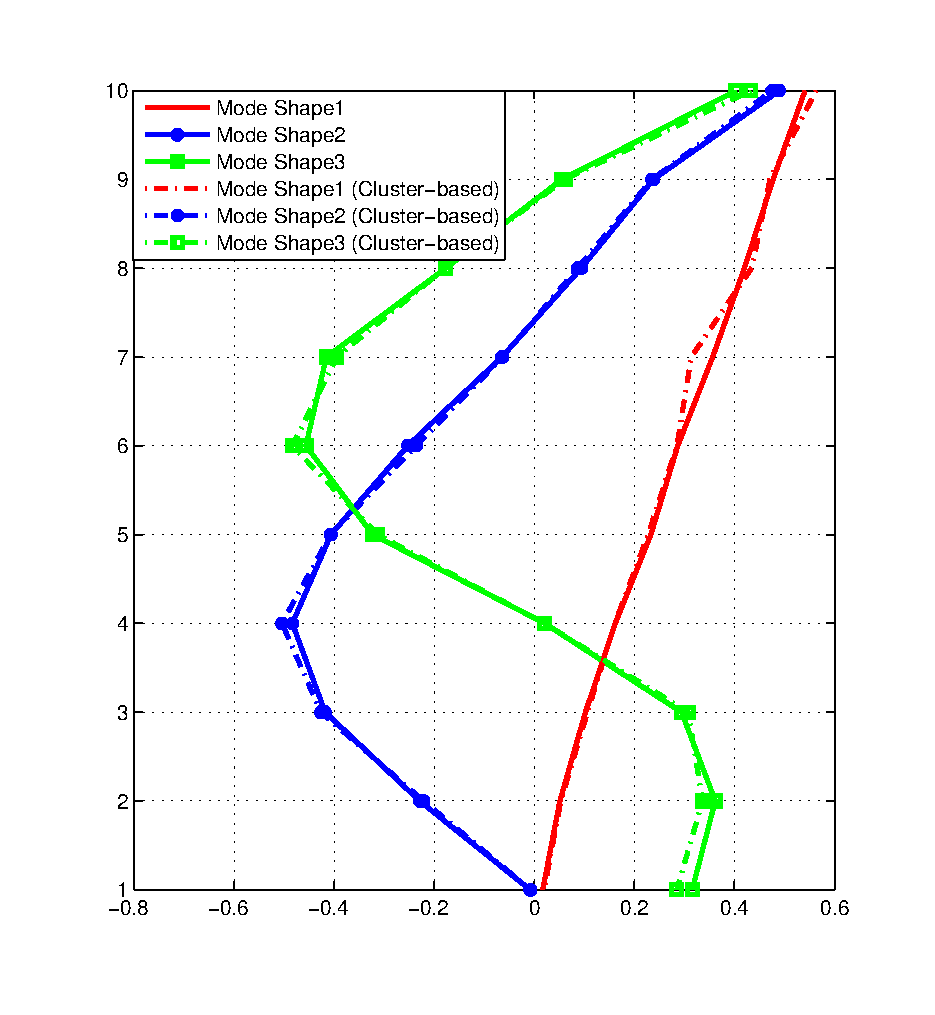
\includegraphics[width=.21\textwidth, height=0.32\textwidth]{TestResults.eps}}
\caption{Clustering and obtained mode shapes}
\label{fig:Clusteringwithmodeshapes}
\end{figure}




%\input{./Implementation}
\section{Conclusion}
\label{sec:conclusion}
In this paper, we presented PSWare, a flexible middleware framework for composite events processing. PSWare uses a flexible architecture where different event detection mechanisms may easily integrated. We described the design of PSWare and explained how it can be customized for different applications. Then we gave two examples of using PSWare. The first one implements a more general composite event algorithm while the second one uses an application-specific event detection approach. Based on our implementation, we performed experiments and demonstrate the effectiveness of PSWare for prototyping and performance comparison.

\bibliographystyle{IEEEtran}
\bibliography{../references/wsn-general,../references/wsn-aggregation,../references/wsn-middleware,../references/wsn-pubsub,../references/edl,../references/pubsub,../references/algorithms,../references/shm}
\end{document}